\documentclass{styles/sig-alternate}

\usepackage{times}
\usepackage{epsfig}
\usepackage{subfigure}
\usepackage{balance}
\usepackage{color}
\usepackage{graphicx}
\usepackage{fancyvrb}
\usepackage{mdwlist}

\newcommand{\ignore}[1]{}
\newcommand{\boldheading}[1]{{\vspace{0.1in}\noindent \bf #1} \hspace{0.06in}}
\newcommand{\somecode}[1]{{\vspace{0.1in}\noindent \bf \tt #1} \hspace{0.02in}}

\renewcommand\topfraction{.95}
\renewcommand\textfraction{.05}
\renewcommand\floatpagefraction{.95}
\renewcommand\bottomfraction{.95}

\hyphenation{cach-ing}
\pagenumbering{arabic}

\makeatletter
\let\@copyrightspace\relax
\makeatother

\begin{document}
\title{Stencil Language and Compiler}
\author{
\alignauthor Greg Faust and Sal Valente\\
\affaddr{CS 6620: Compilers\\
University of Virginia}
}
\maketitle

\begin{abstract}

Parallel hardware is now widely available.  However, writing and optimizing parallel 
programs using sequential languages is difficult and error prone.  
Therefore, it is useful to consider 
new language constructs that make it easier for programmers to express parallel applications
without the need to attend to all the complexity of writing parallel algorithms.  
Here we present a new language in which users can easily 
express computations that involve iterative stencil calculations.  
Such computations form an important subset of parallel algorithms and are 
widely used in scientific, engineering and other important application areas.


Specifically, we present a novel high-level language called Stencil Language (SL).
Using SL, a programmer need only express the central kernel of their 
computation, not an entire parallel program for it.  We have also built a 
translator for SL capable in principal of translating the SL program into code for 
different parallel programming models.  We provide an initial translation into optimized 
code for the C++ extensions of the CUDA programming model for nVIDIA GPUs.  
The optimizer is an extension of an analytical 
model for CUDA stencil applications originally developed by Meng and Skadron \cite{meng}.
The model has been improved to automatically utilize both static and dynamic information 
about the application and the specific GPU environment on which the application is running.
Finally, we validate the compiler and the optimizer through performance evaluation of the resultant code.

\end{abstract}

\section{Introduction}

{\em Iterative stencil loops} (ISLs) \cite{li} are a class of loops
that are commonly used in fields including numerical simulations and
signal processing.  ISLs usually operate on matrices with one, two, or
three dimensions.  An ISL calculation takes an input matrix $m_{in}$
and produces an output matrix $m_{out}$.  The calculation has the
following properties:

\begin{enumerate*}
\item $m_{in}$ and $m_{out}$ have the same number of dimensions and
  the same size.
\item Each value in $m_{out}$ is calculated independently of each
  other value.
\item There is a single function which is used to calculate each value
  in $m_{out}$ regardless of the coordinates of the value.
\end{enumerate*}

For example, say that $m_{in}$ is a two-dimensional matrix.  Say that
the stencil calculation is defined as: ``$m_{out}[x, y] =$ the average
of the north, south, east, and west neighbors of $m_{in}[x, y]$.''
Then this function will be calculated for every cell in $m_{out}$.

The {\em stencil} is the set of cells in the input matrix, relative to
the coordinates of the cell which is being calculated, that is used in
the stencil calculation.  In the above example, the stencil is a set
of four cells: The north, south, east, and west neighbors.

The process of calculating a complete output matrix is called an {\em
  iteration} or a {\em time step}.  At the end of an iteration, we can
take the output matrix $m_{out}$ and use it as the input matrix to the
next iteration.  This loop can continue for as long as necessary.
Some iterative stencil loops are defined to run for a predetermined
number of time steps.  Other stencil loops are defined to run until
the values converge.

Stencil calculations are data parallel.  Since each value is
calculated independently of each other value, the values can be
calculated in any order or at the same time.  If the matrix has $n$
cells and the computer has $k$ processing elements (PEs) available,
then each processor only needs to calculate a block of size $n/k$.  This
partitioning of the matrices among multiple processors is called
{\em tiling}, and the block calculated by a processor is called a
{\em tile}.

When a PE calculates a given tile for many iterations, that PE can
take advantage of both spatial locality and temporal locality.
\begin{itemize*}
\item {\bf Spatial locality.} As a general rule, stencil calculations
  read each input value multiple times.  For example, say that the
  stencil is defined as the cell's left and right neighbors.  When a
  PE calculates the value of a cell at $x=i$, it reads that value of
  that cell's right neighbor at $x=i+1$.  Then, when it calculates the
  value of a cell at $x=i+2$, it reads that cell's left neighbor, which
  is the value at $x=i+1$ again.  Thus, a PE can optimize this
  computation by keeping input values in a local cache.
\item {\bf Temporal locality.} If a PE generates an output value
  during iteration $x$, then that PE can use that value as an input
  value during iteration $x+1$.
\end{itemize*}

Unfortunately, stencils along the boundary of a tile cannot find all
of their input values in the local processor cache.  These stencils
must obtain values that were computed on other PEs.  The regions of
data that must be exchanged are called {\em halo} regions.  As a
result of this exchange, ISL algorithms may spend considerable time
stalled due to communication and synchronization delays.

\begin{figure}
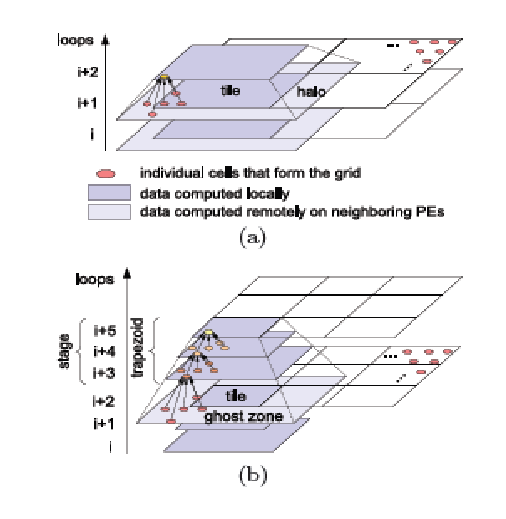
\includegraphics[clip,trim=.75in 7in 4.75in 0.75in,width=3.3in]{StencilDiagram}
\caption{(a) Iterative stencil loops and halo regions.  (b) Ghost zones help
reduce need for global synchronizations.  Note: this figure was drawn by Meng, 
and is reprinted here with the authors' permission.}
\label{fig:trapezoid}
\end{figure}

A solution to this problem is to include a {\em ghost zone} in each
tile.  A ghost zone is a perimeter around the tile which overlaps
neighboring tiles.  The overlap allows each PE to generate its halo
regions locally for one or more iterations.  Specifically: Say that a
processor is responsible for calculating a tile with $n$ cells.  As
input, the processor is given a larger tile with values in those $n$
cells and also in $x$ halo regions around those cells.  The processor
can execute $x$ iterations without communicating with any other
processor, and it will end up with valid values in the $n$ cells in
the output tile.

We call the number of halo regions in the ghost zone the {\em pyramid
  height}.  Figure~\ref{fig:trapezoid} shows the pyramid of
progressively smaller tiles.

In the paper ``Performance Modeling and Automatic Ghost Zone
Optimization for Iterative Stencil Loops on GPUs,'' \cite{meng}
Jiayuan Meng and Kevin Skadron wrote:

\begin{quote}
Ghost zones pose a trade-off between the cost of redundant computation
and the reduction in communication and and synchronization between
PEs.  This trade-off remains poorly understood.  Despite the ghost
zone's potential benefit, an improper selection of the ghost zone size
may negatively impact overall performance.
\end{quote}

Meng and Skadron examined the problem of writing efficient ISL code in
the CUDA language to run on an nVIDIA GPU.  They defined a mathematical
model for calculating the optimal ghost zone size.  Unfortunately, the
model is hard to use.  It has roughly a dozen parameters, and some of
them are difficult to calculate both at compile time and at runtime.

To summarize, writing efficient ISL code is difficult for these reasons:
\begin{itemize*}
\item The code must use tiling to take advantage of spatial locality.
  Writing the tiling code can be confusing because of the need to 
  properly handle a lot of edge cases.  In addition, calculating the 
  optimal tile size can be challenging, yet is a critical factor 
  in the performance of the application.
\item The code must use ghost zones to avoid global synchronization and 
  communication delays.  Calculating the optimal ghost zone size is 
  non-trivial.  In addition, the code to handle the ghost zones is
  messy and error prone.
\item The code must be optimized for a particular environment.  The
  optimal ghost zone size on an old GPU might be different from the
  optimal size on a new GPU which might be different from the optimal
  size on a multicore CPU.
\end{itemize*}

The goal of our research is to define and create tools which make it
easy to write ISL code.  The programmer of a stencil calculation
should not need to write code to calculate the optimal ghost zone
size.  In fact, he should not need to write any code that is in any
way related to tiling or ghost zones.  Nor should he need to write
code to optimize spatial or temporal locality for one or more
environments or architectures.  It should be possible to implement an
efficient ISL simply by describing the stencil and the stencil
calculation.

We have achieved these goals.  Our contributions are as follows:
\begin{itemize*}
\item We have defined a {\em stencil language}.  This is a formal
  high-level language in which a programmer can describe an ISL
  computation.  By design, a description written in the language must
  include all of the information necessary to calculate the correct
  results, and none of the information that would tie its performance
  to a particular architecture.
\item We have created a stencil language compiler.  The front-end of
  the compiler parses the stencil file.  The back-end outputs
  efficient CUDA code.
\item The CUDA code calculates the optimal ghost zone size.  It
  extends the model defined by Meng et al.
\item We have refined the model to collect as much information as
  possible dynamically at runtime.  This allows the generated code to
  calculate good values on a variety of GPU cards, and it should allow
  the code to continue to work well with future hardware.
\item We have designed our compiler so that it can be extended with
  multiple back-ends.  Based on a single source file, it could output
  efficient code for CUDA or OpenMP or pthreads or other environments.
\end{itemize*}

The remainder of this paper is organized as follows.  Section 2
discusses related work.  Section 3 is the complete definition of our stencil
language.  Section 4 presents the design and implementation of our
stencil language compiler.  Section 5 discusses the CUDA code which is
generated by the compiler, including the code which calculates the
optimal ghost zone size.  Section 6 discusses the performance of the
generated code.  It contains our experimental setup and results.
Section 7 concludes.

\section{Related Work}

Zhiyuan Li and Yonghong Song may have been the first to use the term
{\em iterative stencil loops} \cite{li}.  They developed a compiler
framework for these loops that used tiling to improve temporal data
locality.  Their work was intended to be run on a uniprocessor, so
they did not face any communication costs and they did not consider
ghost zones.

We are not the first to create a stencil compiler.  A group at Harvard
created a stencil compiler for the Connection Machine CM-2 massively
parallel architecture \cite{cm2}.  The stencil expression was
expressed for their compiler in a ``microcode'' which was specific to
the CM-2 architecture.

Shoaib Kamil et al. studied the effects of tile size and time skewing
to increase memory locality on the Itanium2, Opteron, Power5, and Cell
\cite{kamil}.  They concluded that controlling tile size and data
locality reuse across time slices is critical to performance.  In
addition, they concluded that when hand optimizing, better performance
is achievable on the Cell because of the users' explicit control of
the memory hierarchy.  We optimize use of CUDA's explicit memory hierarchy 
through our use of shared memory.  In addition, we also optimize tile
size and ghost zones.  However, our pyramid height is always in the time
dimension; we have not investigated use of time slewing.

Paulius Micikevicius from nVIDIA explored the hand coding of stencil
applications on CUDA, and in particular the desired sizes of ghost
zones around the array tiles \cite{Micikevicius}.  He also
investigated using asynchronous data transfers and computations for
array sizes too large to fit in GPU global memory.  In a somewhat
related area, Vasily Volkov investigated in great detail hand
optimizations of CUDA programs involving parallel operations on large
arrays \cite{volkov}.  For our project, we have done manual
optimizations of a subset of those presented by Micikevicius and Volkov so
that the user of our compiler does not need to be aware of them.  We have
no support for arrays too large to fit into the devices global memory,
nor do we use asynchronous data transfers.

Several attempts have been made to build simplifying layers on top of
the CUDA language.  At Purdue, they built a source-to-source
translator for OpenMP to CUDA \cite{openmp}.  OpenMP is a
standards-based set of language extensions targeted at expressing
parallel computations on shared memory architectures.  OpenMP can
express a significantly wider range of parallel computations then that
which can be expressed by our stencil language.  However, this also
means an OpenMP translator cannot include stencil application specific
optimizations as we do.

CUDA-lite is a general purpose source-to-source translator for
automatically optimizing CUDA programs \cite{cudalite}. The user
expresses his program in CUDA syntax, but using only the largest, 
most general, and easy to use level of the CUDA memory hierarchy; the global
memory space.  Therefore, it is easier to write CUDA programs that solely use
this memory space than to write programs optimized for the
smaller, faster memory spaces.  With CUDA-lite, the user includes some
additional pragmas in his code that gives hints to CUDA-lite about the
size, shape, and access of the global memory arrays.  Then CUDA-lite
generates a CUDA program that takes advantage of the special memory
spaces, generally resulting in a factor of 3X speedup.  Our compiler
also optimizes for use of shared memory.
However, they do no stencil application specific optimizations, and cannot 
take advantage of performance gains from the use of ghost zones.

\section{Stencil Language}

\subsection{Syntax}

A stencil language file is a plain text line-oriented file that
contains a set of key-value pairs.  The key and value are separated by
whitespace.  A key is an alphanumeric string.  A value can be:
\begin{itemize*}
\item an integer
\item a name comprised of alphanumeric and underscore characters
\item a list of names, inside parentheses, separated by commas
\item a block of C code inside of curly braces
\end{itemize*}
Comments start with {\tt //} and go to the end of the line.

\subsection{Content}

\begin{itemize}
\item {\bf NumDimensions} -- A stencil may have 1, 2, or 3 dimensions.
\item {\bf StencilSize} -- The size of the stencil in each dimension.
  If the stencil size is 1 in the $x$ dimension, then the value of the
  cell at $(x, y)$ may be based on the previous iteration's values of
  the cells in the $x-1$ and $x+1$ coordinates.
\item {\bf DataType} -- The data may be 32 bit or 64 bit integers or
  floating point numbers.  The values are {\tt int}, {\tt int64}, {\tt
    float}, and {\tt double}.  Values may be signed or unsigned.
\item {\bf FunctionName} -- The name of the function that will be exported
  from the generated CUDA source file.  The first argument to the function,
  {\tt data}, will be a matrix of the specified data type with the
  specified number of dimensions.  As input to the function, {\tt
    data} must contain the initial state of the problem.  It must
  contain valid data in each cell.  As
  output from the function, it will contain the final data.  The next
  $n$ arguments to the function are the input sizes in each dimension.
  The next argument is the number of iterations to run.
\item {\bf ScalarVariables} -- A list of numeric variables that will
  be arguments to the exported function after {\tt data, x, y, z,
    iterations}.  The caller will pass these arguments to the
  function, and then the stencil calculator will be able to use these
  variables (read-only) in its calculations.
\item {\bf CellValue} -- A block of C code that will be run for every
  cell in the data set in every iteration.  The code has access to the
  following variables and functions:
\begin{itemize}
\item {\tt x, y, z} -- The coordinates of the current cell in each
  dimension.
\item {\tt iteration} -- The iteration number.  Since iteration 0 is
  given as input, this code will first be called with {\tt iteration}
  = 1.
\item {\tt input\_size} -- a structure with {\tt x}, {\tt y}, and {\tt
  z} fields, containing the total size of the input
\item All variables listed in the {\bf ScalarVariables} field.
\item {\tt get(...)} -- a function that efficiently returns values
  from the stencil from the previous iteration.  The parameters are
  relative to the current cell.  For example, in a two-dimensional
  stencil, the west and east neighbors can be retrieved with {\tt
    get(-1, 0)} and {\tt get(1, 0)}.
\end{itemize}
The block of code returns the new cell value.
\item {\bf EdgeValue} -- A block of C code that returns the cell value
  of cells that are outside the bounds of the input.  This code has
  access to the same variables as the {\bf CellValue} code.  Note that
  at least one of {\tt x}, {\tt y}, or {\tt z} will be out of bounds
  -- it will be either less than zero or greater than or equal to the
  size of that dimension.  This code may not use the {\tt get()}
  function.  Instead, it can access the {\tt value} variable, which
  will contain the value of the nearest cell in bounds from the
  previous iteration.
\end{itemize}

\subsection{Unnamed Data}

The generated CUDA source file will export two functions.  One of the
functions will have the given function name.  The other function will
have the function name appended with {\tt SetData}.  For example, if
the stencil language file says:
\begin{verbatim}
FunctionName runStencil
\end{verbatim}
then the generated CUDA source file will export these two functions:
\begin{itemize*}
\item {\tt runStencil()}
\item {\tt runStencilSetData()}
\end{itemize*}

\noindent The SetData function takes two arguments:
\begin{enumerate*}
\item An array of elements of the specified data type
\item The number of elements in the array
\end{enumerate*}
If a program calls the {\tt runStencilSetData()} function with an
array, and then the program calls {\tt runStencil()}, then the stencil
calculator will have read-only access to this data in the array.  The
{\bf CellValue} code can access the $i$th read-only data element by
calling {\tt read(i)}.

\subsection{Example Source File}

Figure~\ref{fig:hotspot} shows a stencil language description of the
``hotspot'' calculation.  This code calculates the temperature
patterns in a two-dimensional microchip where the current state is a
function of the previous state, the edge values, and a two-dimensional
read-only ``power usage'' matrix.

\begin{figure}
\begin{small}
\begin{verbatim}
NumDimensions 2
StencilSize (1, 1)
DataType float
FunctionName runHotspot

ScalarVariables (
  float Rx, float Ry, float Rz
}

CellValue {
  float pvalue, value, term1, term2, term3, sum;
  pvalue = read(y * input_size.x + x);
  value = get(0, 0);
  term1 = (get(0, 1) + get(0, -1) - value) / Ry;
  term2 = (get(1, 0) + get(-1, 0) - value) / Rx;
  term3 = (80.0 - value) / Rz;
  sum = pvalue + term1 + term2 + term3;
  return(value + sum);
}

EdgeValue {
  return value;
}
\end{verbatim}
\end{small}
\caption{The hotspot.sl stencil language file.  This example
  shows a description of a two-dimensional stencil calculation where
  the value of each cell is based on the values of that cell's
  immediate neighbors.  The read-only data is interpreted as a
  two-dimensional matrix which indicates that some areas of the chip
  inherently run hotter then other areas.}
\label{fig:hotspot} 
\end{figure}

\section{Stencil Language Compiler}

We implemented the stencil language compiler in less than 600 lines of
Java code.  This is what it does:
\begin{enumerate*}
\item Convert a stencil language file into a token stream
\item Parse the token stream into a symbol table
\item Read a plain text template file
\item Output a new file which contains the template integrated with
  the stencil description
\end{enumerate*}

Step 1 is implemented by {\tt Tokenizer.getToken()}.  A token is
either a string of alphanumeric characters or any symbol token that's
in the language such as parentheses, commas, etc.  Also, the tokenizer
can recognize comments and blocks of C code.

Step 2 is implemented by {\tt Stencil.parse()}.  It runs a loop that
reads a key and then parses a value, which may be an integer, a
string, a list, or a block.  The parser verifies that the key is
defined by the language and that the value has the right type for that
key, and then it adds the key value pair to a symbol table.

Step 3 is implemented by the creator method of the {\tt Template}
class.  It stores the template text in the Template instance.

Step 4 is implemented by {\tt Template.applySymbolTable()}.  It looks
for instances of {\tt @name@} in the text.  For each instance that it
finds, it looks up {\tt name} in the symbol table, and it replaces the
variable with the value.

This design is flexible.  It can easily support multiple architectures
and optimizations.  We have written templates for CUDA code for 1-D,
2-D, and 3-D stencil calculations.  These templates are written such
that the {\bf CellValue} code can be dropped-in unmodified.  The code
in these templates is optimized for shared memory usage, and it
calculates the optimal ghost zone size.  We have also written a
template which does not use shared memory or ghost zones, 
so that we could compare
its performance to that of the optimized templates.

We are confident that an OpenMP template could be written without
requiring any changes to either the stencil language or the compiler.

\section{Generated CUDA Code}

\subsection{CUDA Architecture Overview}

The CUDA programming model is a set of extensions to the C++ language that
the nVIDIA Corporation created to allow for the use of
their graphics cards (GPUs) to be used for general purpose parallel 
computing.
The model involves using the GPU as a co-processor for the CPU.
A control thread on the CPU does some of the work for the application, 
but can call on the GPU to perform certain parallel calculations
when desired.  The parcel of work for the GPU is called a {\em kernel}
and usually represents an inner loop that exhibits large degrees of
data parallelism.  The code for the kernel is written for one thread
as if it were the only thread running, except that it is given a
thread-id from which it can compute its position in the collection of
threads launched in the kernel invocation.  While the kernel code can
be written rather simply for simple applications, the optimal use of the
GPUs resources requires significantly more effort and complexity.

One source of the complexity for optimizing kernels comes from the rather
arcane memory hierarchy on the device due to its primary use as a graphics
accelerator.  The hardware of the GPU is organized into a collection of PEs
each of which is a SIMD core with 8 scalar processing elements.  Both the 
organization of the GPU into separate PEs, and the related variety of
different types of memory, are made visible to the kernel author.

When calling a kernel, the user must specify the organization of the
resultant threads into thread blocks, including the 3 dimensional shape
of the thread block.  Current GPU cards support up to 512 threads per
block.  A thread block will be allocated by the CUDA runtime system
to a particular PE on which it will execute.  Each PE has a modest amount
of very fast {\em shared memory} that can be shared by threads in a thread block, but
not be accessed by any other thread blocks.  For the purposes of this paper,
the only other memory structure available to threads running on the GPU is
a large global memory accessible by all threads on the device.  However, this
large memory is not cached, and has access latencies of around 400 to 600 clock
cycles.  Therefore, a critical optimization technique for kernel authors is to
properly group threads into blocks that can use the shared memory to best effect.

In addition, the CUDA model does not support any global synchronization primitive
between thread blocks during a kernel execution.  Instead, global synchronization
events require the completion of all running thread blocks and a return of control to 
the CPU control thread.  A further complication is that no data stored in the 
shared memory of a PE is persistent across kernel calls.
Such global synchronization events are therefore very costly.

The implication of this model for stencil applications is that the kernel
author must be intimately familiar with the details of the CUDA runtime
system in order to organize work units into thread blocks in such a way
that usage of shared memory is maximized, and accessed to global memory
are minimized.  Key decisions in this allocation are precisely the
tile size and pyramid height of the stencil calculation that the optimization
model is designed to make.  In order to accurately make such decisions it must
be able to predict the latencies of the various operations involved in the kernel's
calculations and memory accesses on the GPU device upon with the application will run.

\subsection{ISL Calculations}

This section describes how the hand-written CUDA code works.  This
code can be found in the file {\tt template3d.cu}, and also in the 1-D
and 2-D versions of that file.

The main function in the template is a C function (as opposed to a
CUDA kernel).  First, it calculates the tile size and the ghost zone
size.  Then, it copies the input matrix from system memory into GPU
memory.  Finally, it runs a loop in which it invokes the CUDA kernel
to calculate the output matrix from the input matrix.  It runs this
loop for the specified number of iterations, divided by the pyramid height.

Each tile is processed by a single CUDA thread block, and each cell in
the tile should be owned by a single thread.  A CUDA thread block can
have up to 512 threads, so the 3-D tile is defined as $8 \times 8
\times 8$.  The 2-D tile is $22 \times 22$, and the 1-D tile is 512
cells long.  This is the size of the input tile, including ghost zone
cells.  The size of the output tile will be smaller.

Here's what the CUDA kernel does:

The thread calculates the $(x, y, z)$ coordinates of the cell in the
matrix that it owns.  It copies that cell's value from the input
matrix into the thread block's shared memory.  After each value has
been copied into shared memory, the threads that own cells in the
outermost halo go to sleep.  Those threads have completed their work.
Each other thread calculates the new value for its cell.  For each
cell in its stencil, the thread gets the cell value from shared
memory.

If the pyramid height is greater than one, then the threads continue
running.  Each thread copies the value that it just computed into
shared memory.  Then, the threads in the second outermost halo go to
sleep.  They're done.  The remaining threads calculate new values.
This process continues for the number of iterations specified by
pyramid height.

When this process is complete, if a thread owned a cell that was not
in the ghost zone, then that cell copies the final value into device
memory.  If a thread owned a cell that was in the ghost zone, then
that thread does not need to do anything, since we are guaranteed that
some thread in some other thread block owned the same cell, and that
other thread will calculate the new value and write the value into
device memory.

Inside of the CUDA kernel, the program calls the user-specified
CellValue code to calculate new cell values, and it calls the
user-specified EdgeValue code to get stencil values for cells along
the edges of the matrix.

If an array of read-only ``unnamed data'' was specified, then the
program copies that data into device memory before the program enters
the CUDA kernel.

\subsection{Ghost Zone Size Calculation}

As mentioned previously, the performance of stencil applications on parallel hardware 
is critically dependent on the proper relationship between tile size and ghost zone size,
or equivalently, the pyramid height (PH).
In order to calculate the optimal PH,
we have extended the analytical model for CUDA programs that was written by Meng using MatLab.  
He developed a complex analytical model for CUDA programs that utilizes information from a variety of sources.
From this information, it calculated the expected runtime (in GPU clock cycles) for the program.

First, important information about the stencil application itself is needed.  Some of this information is 
static such as the number of dimensions of the data, the size of the stencil (halo), 
the number of global memory accesses required during movement of tile data into shared memory, 
and the number of global accesses for read-only 
data required during each cell value calculation.  Other information is dynamic such as the data set size
and the number of instructions that each thread must execute
(1) in the shared memory setup portion of the kernel, and (2) in the cell value calculation of the kernel.  
Since he did not implement any code annotations for the stencil applications, 
many of the application specific parameters were hand coded into the MatLab code for the four particular 
applications he chose as his test cases.  In addition, the instruction count information was gathered 
by using the CUDA profiler on hand-coded implementations of the test applications, and fed to the model by hand.

Second, information about the properties of the target CUDA GPU are important.  
This includes the number of PEs, 
the number of concurrent blocks that can run on a PE, the number of threads allowed per block (tile), 
the time required for the GPU to perform a global synchronization, 
and several parameters of the GPU memory performance.  
These values were acquired from a number of places including hand coding of some parameters 
based on the published characteristics of a few specific models of GPU, 
and some achieved by data regression (curve fitting) of runtimes from specific applications.

We have modified and/or improved this model in several important ways.  
First, we ported the model from MatLab to C++ so that we could include it in the application 
to perform the optimization at runtime.  This has several advantages including gathering 
information about the run time aspects of the program such as data size, 
and gathering specific information about the current execution environment.  
The latter allows the program to be run on different GPUs without recompilation, 
and better optimized for the specific characteristics of the particular hardware, 
not just the architectural features of the hardware.  While this means that the time 
to perform the optimizations is included in the runtime for the program, the difference 
in runtimes for the wrong optimizations will generally dwarf any cost of calculating the 
optimizations themselves.  In addition, stencil applications typically take many 
iterations to converge, allowing more runtime over which to amortize the optimization costs.

Second, the static and architecture-independent application specific information about the 
dimensions of the data space, the stencil size, etc. now come directly from the SL specification for the program.  
These are compiled into the generated code for the ISL calculation.

Third, the rest of the application specific information is acquired dynamically at runtime.  
This includes the data set size, and the other parameters that previously came from profiling 
such as the latency of the thread setup time and cell value calculation time.  The latter two 
numbers are acquired by running the application with PH of 1 and 2. From these numbers, 
the setup and cell value calculation times are easily computed.  Currently we throw away the actual 
application computation performed during these data gathering runs of the kernel.  
In the future, the time spent gathering this information should also result in the 
completion of the first 3 iterations of the computation.

Fourth, the information about the GPU device the application will run on is gathered through calls
to various informational functions provided in the CUDA runtime libraries.  In particular, we can acquire 
the number of PEs, the number of concurrent blocks per PE, and the maximum number of threads allowed 
per block in this manner.  In addition, one can query the CUDA runtime system for the number of 
thread per block for the actual kernel of the running application.  This can sometimes result in 
tighter restrictions on the number of allowed threads per block if, for example, the kernel requires 
more resources from the device than it can provide at the architecture maximum number of thread per block.  
This is particularly true for CUDA kernels that use a lot of registers.  
Knowing this number is critical to the optimization.  That is because all stencil applications 
will always run better with a larger tile size.  Since the number of thread per block determines the tile size, 
knowing this number precisely allows for the optimizer to always pick the largest tile size that the current GPU can handle.
Future GPUs may allow the number of threads per block to increase beyond 512.  Gathering this information at run time
allows generated code to calculate the optimal tile size for such cards without regeneration by the SL compiler.

Fifth, the time required for a global synchronization on the device is acquired by 
running a null kernel on the device with the same data set size parameters as are required to run the actual kernel.

Finally, Meng et al. originally did a manual gradient descent on runtimes to determine 
the best PH and tile size.  Since we can determine the best tile size as described above, 
we do an automatic gradient descent starting at PH of 1, 
and continue calculating the model latency until it is higher than the previous one, 
then stop and use that PH for the remainder of the application iterations.

\section{Experimental Results}

Our primary goals for this research were to define a stencil language, provide a compiler for it, 
and to statically and dynamically optimize the generated programs in terms of the use of GPU shared memory, 
tile size and PH for the target set of GPU architectures for which the performance model was 
originally developed.  It was not our goal to improve the performance of the optimizer to a broader set of 
nVIDIA GPU cards.  Therefore, we restricted our testing to the original target environment for the optimizer.
Out testing environment contains 2 Intel Core2 Extreme X9770 processors running at 3.2GHz with 6MB of L2 cache 
and 4GB of DRAM.  The OS is Linux 2.6.24.  The installed graphics card is a GTX-280 nVIDIA GPU running 
version 2.2 graphics driver.  The GTX-280 has 30 PEs each of which has 8 SIMD cores and can handle up to 8 
concurrent running blocks, with maximum block size of 512 threads.  It has a clock speed of 1.3GhZ, and 1GB of
global memory.  All code was compiled with the nVIDIA provides NVCC compiler driver which in turn 
calls GNU tools for compiling C++ code and linking.  The installed GNU tools were version 4.2.4, and all code was
compiled with -O3.

For our test cases, we use the same four stencil applications as Meng et al. did in his original study.  
They are described below.
All of the graphs of runtimes vs. PH have the same basic curve.  Very low PHs are not
large enough to take advantage of all available spatial and temporal locality, and perform worse than larger
PHs.  However, beyond some optimal PH, the runtimes again increase due to the overhead
of all the ghost zone calculations that are thrown away at the global synchronization point.  Another way to
see this trade-off is that with increased PH, the number of threads per tile that calculate final cell 
values drops off at twice the size of the stencil per dimension per step in PH (see Figure~\ref{fig:trapezoid}).  Therefore, 
for very larger PHs the effective tile size gets smaller, and the total number of tiles, and therefore
also the total number of threads, increases.  Eventually, in the limiting case, the PH is so high that 
{\em no} useful cell values are calculated!  Near this extreme, run times increase exponentially.  For these reasons, all of the graphs
of runtimes vs. PH will be bowl shaped.

\subsection{\em ``Pathfinder''}

The first test case is a 1D stencil application called {\em ``Pathfinder''} that performs a dynamic programming calculation 
of the lowest cost of any vertical path through a two dimensional grid of data.  
The 2D input data set is read-only data during the CellValue computation.  
Each iteration of the main loop calculates the min costs down another row in the 2D grid.
The tiles are horizontal slices across the columns of the 2D grid.  A valid path is one which varies by at most one cell 
in each step from row to row.  Therefore, the stencil size is 1.  As this is a 1D application,
the current theoretically possible PHs vary from 1 to 255.  
Figure~\ref{fig:pathfinderTimes} shows the runtimes vs. PH for pathfinder for
row width of 100,000 and 400,000.  As with all the applications, these large sizes are chosen to ensure
that the GPU is saturated with threads.  Meng et al. originally also ran this at row widths of 700,000 and 1,000,000 as did we.
However, the latter two data sets have been left out of the chart, as they have the same shape, and are enough
larger in magnitude that their inclusion would compress the detail that is most important to see.  For the same
reason, PHs above 235 are not shown as they raise so dramatically that they would again compress
the interesting part of the curve.  


Notice that the valley for the main portion of this curve is very shallow.  Therefore, it 
is hard for the model to accurately predict the exact best PH.  And in fact, our model does not.  For the 100,000 column data set,
the measured best PH is 16, our model predicts 18 with a resultant loss of performance of 2.79\%.  For the 400,000 column data set,
the measured best height is 17, our predicted height is 21, with a resultant loss of performance of 2.74\%.  For the 700,000 column data set,
the measured best height is 12, while our predicted height is 20, but still this only results in a performance loss of 1.0\%.  Finally, for the
million column data set, the measured best height is 14, while we predict 19, with a resultant loss of 0.99\% in performance.  From these results, one
can see that the shape of the interesting part of the curve is so flat that precise PH prediction is not necessary to result in very positive results.
For comparison, the naive use of a PH of 1 for the 1,000,000 column data set would result in a performance loss of 43\%.

\begin{figure}
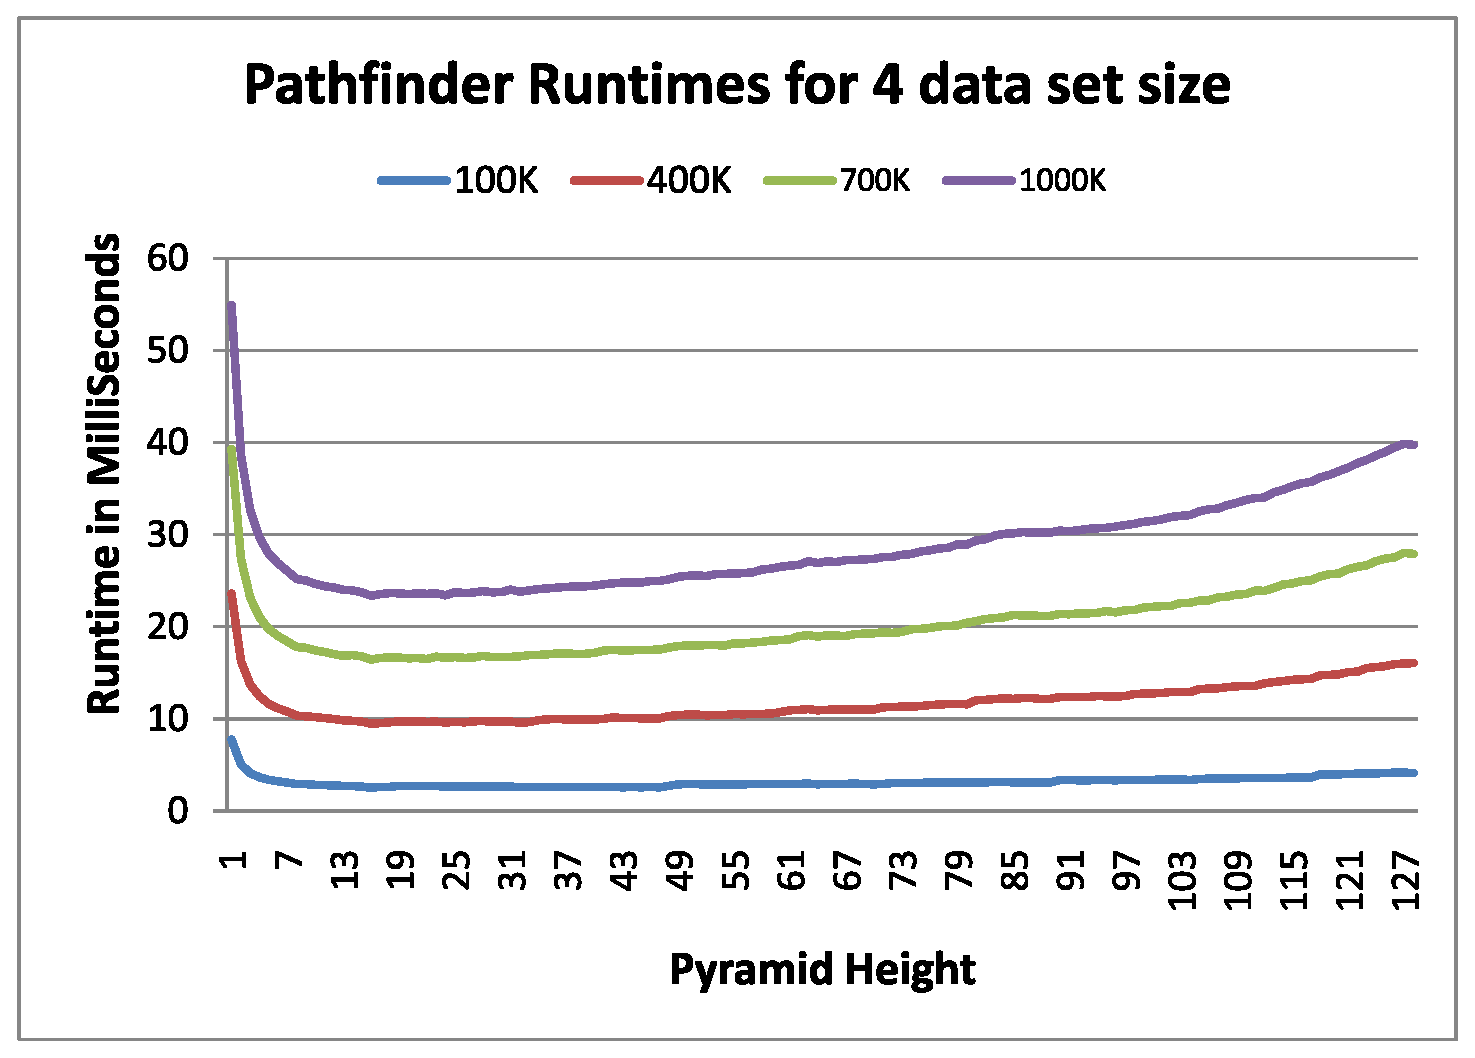
\includegraphics[clip,trim=1in 1in 1in 1in,width=3.3in]{PathfinderTimingData}
\caption{This chart shows the actual measured runtimes for the Pathfinder 1D stencil application vs. PH.
As can be seen, the lowest portion of the curves are very flat.  Therefore, even though our analytical model did not 
accurately pick the best PH for any data set size, the resultant performance was between 0.99\% and 2.79\% of optimal.}
\label{fig:pathfinderTimes}
\end{figure}

\subsection{\em ``HotSpot''}
The second test case is a 2D stencil application called {\em ``HotSpot''}.  
The stencil language description for this application is show in Figure~\ref{fig:hotspot}.
The application calculates an ordinary differential equation that models heat dissipation in a conductive material.  
In this case, the modeled material is the silicon substrate of a computer chip \cite{hotspot}.
On each time step of the computation, the heat generated by the chip components are injected through the modeled substrate.  
This is constant read-only data read for each cell on each iteration.  As this is a 2D application, 
the current theoretical maximum square tile size is 22x22.
This implies a possible PHs range from 1 to 10.  The resultant runtimes vs. PH are show in
figure~\ref{fig:hotspotTimes}.  As can be seen, the the 4 data set sizes, the optimal PH is 2.  And that is also the height calculated by
our optimizer.  Again we have removed the value for PHs above 6 as they rise dramatically and would compress the important portion of the curve.

\begin{figure}
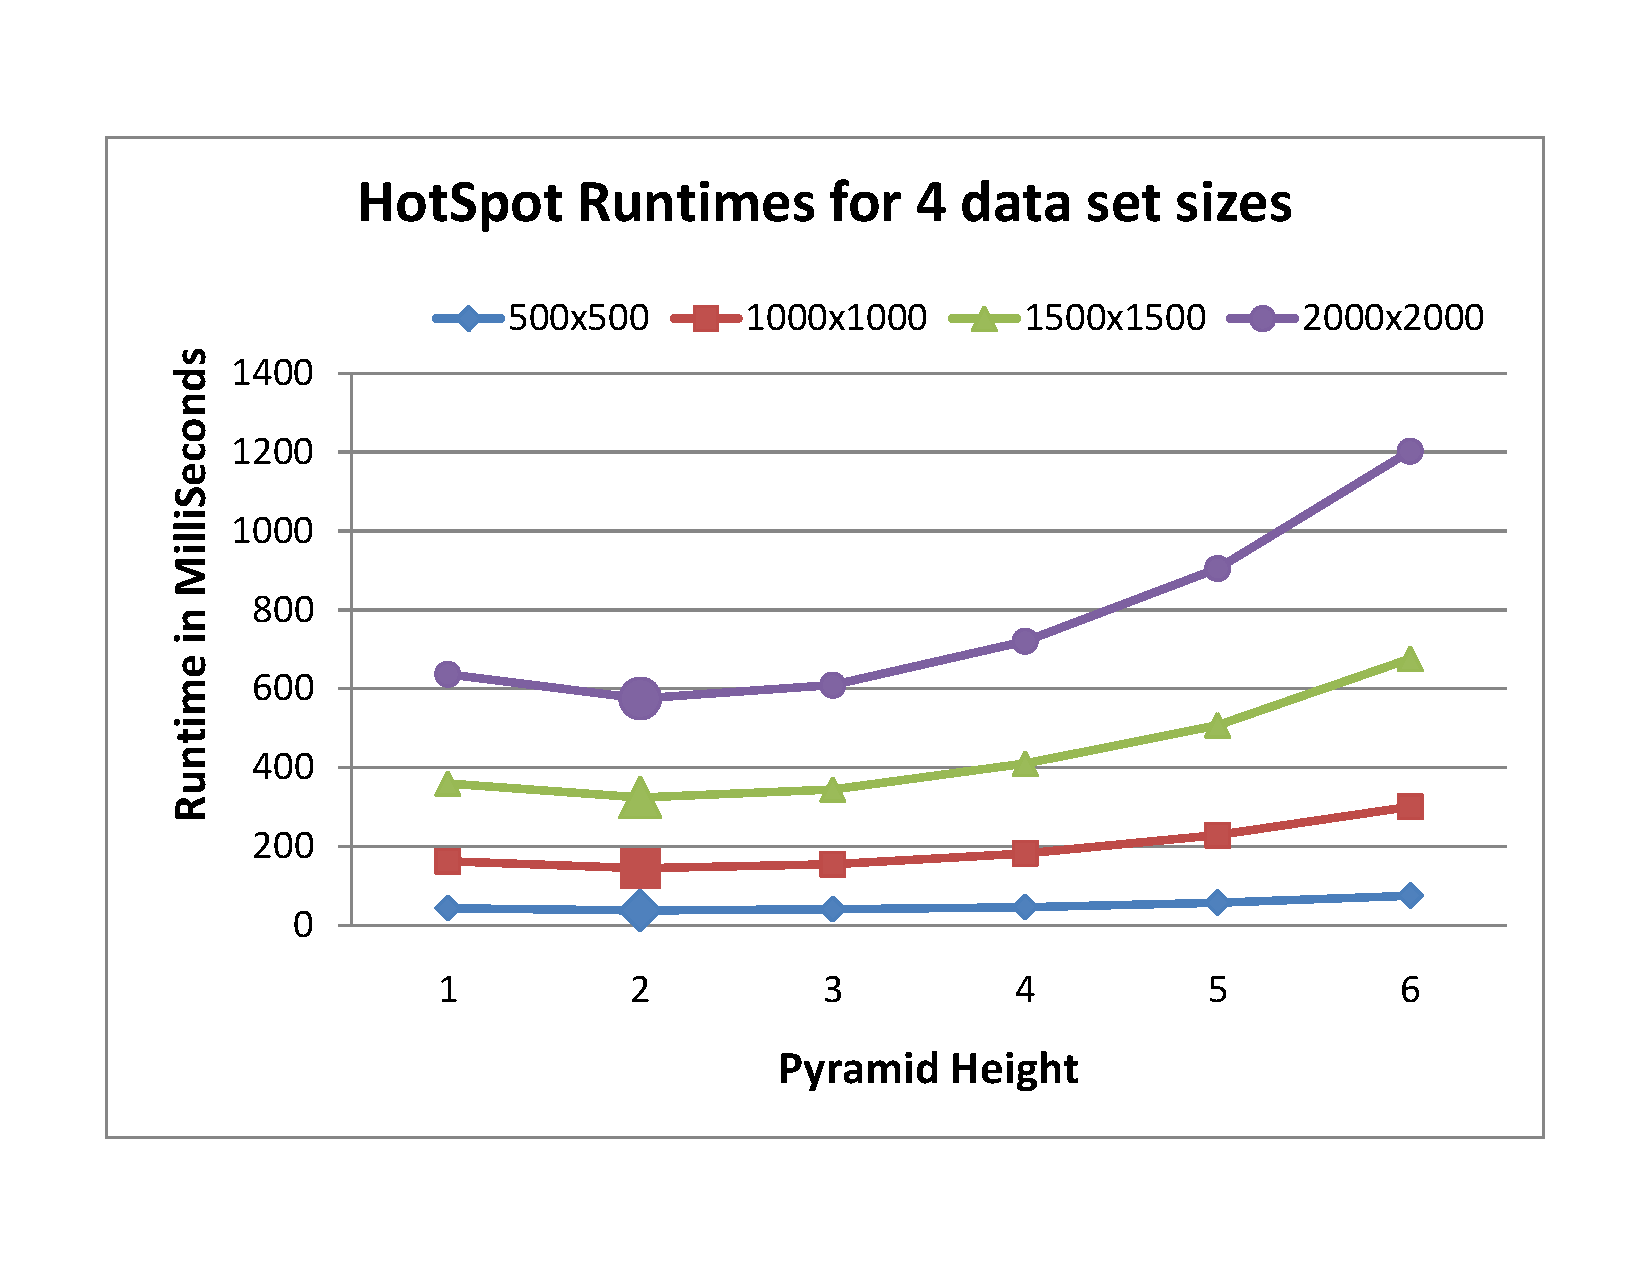
\includegraphics[clip,trim=1in 1in 1in 1in,width=3.3in]{HotSpotTimingData}
\caption{This chart shows the actual measured runtimes for the HotSpot 2D stencil application vs. PH.
As can be seen, the curve is bowl shape with a noticeable low point at PH 2.  The effect is more pronounced
with greater data set sizes.  Our optimizer picked the correct PH of 2 for all these data sets.}
\label{fig:hotspotTimes}
\end{figure}

\subsection{\em ``Plate''}
The third test case is another 2D stencil application called {\em ``Plate''}.  It is very similar to and replaces the 
{\em ``Poisson''} application from the original test suite.  It also models heat transfer in a plate but this time, the heat 
injection into the system is modeled as coming in from the edge of the plate, not distributed throughout the plate.  The makes the application
different from HotSpot in two important ways.  First, there is no required read of global data in each time step.  Second, it gave us an opportunity
to use the {\bf EdgeValue} capability of the SL to inject the heat at the plates edge.  Again the maximum square tile size is 22x22 and valid PHs are 1 through 10.  
The graph of runtimes vs. PH is very similar to HotSpot and shown in Figure~\ref{fig:plateTimes}.
Again both the optimal PH and our model's predicted PH is 2 for all four data set sizes.

\begin{figure}
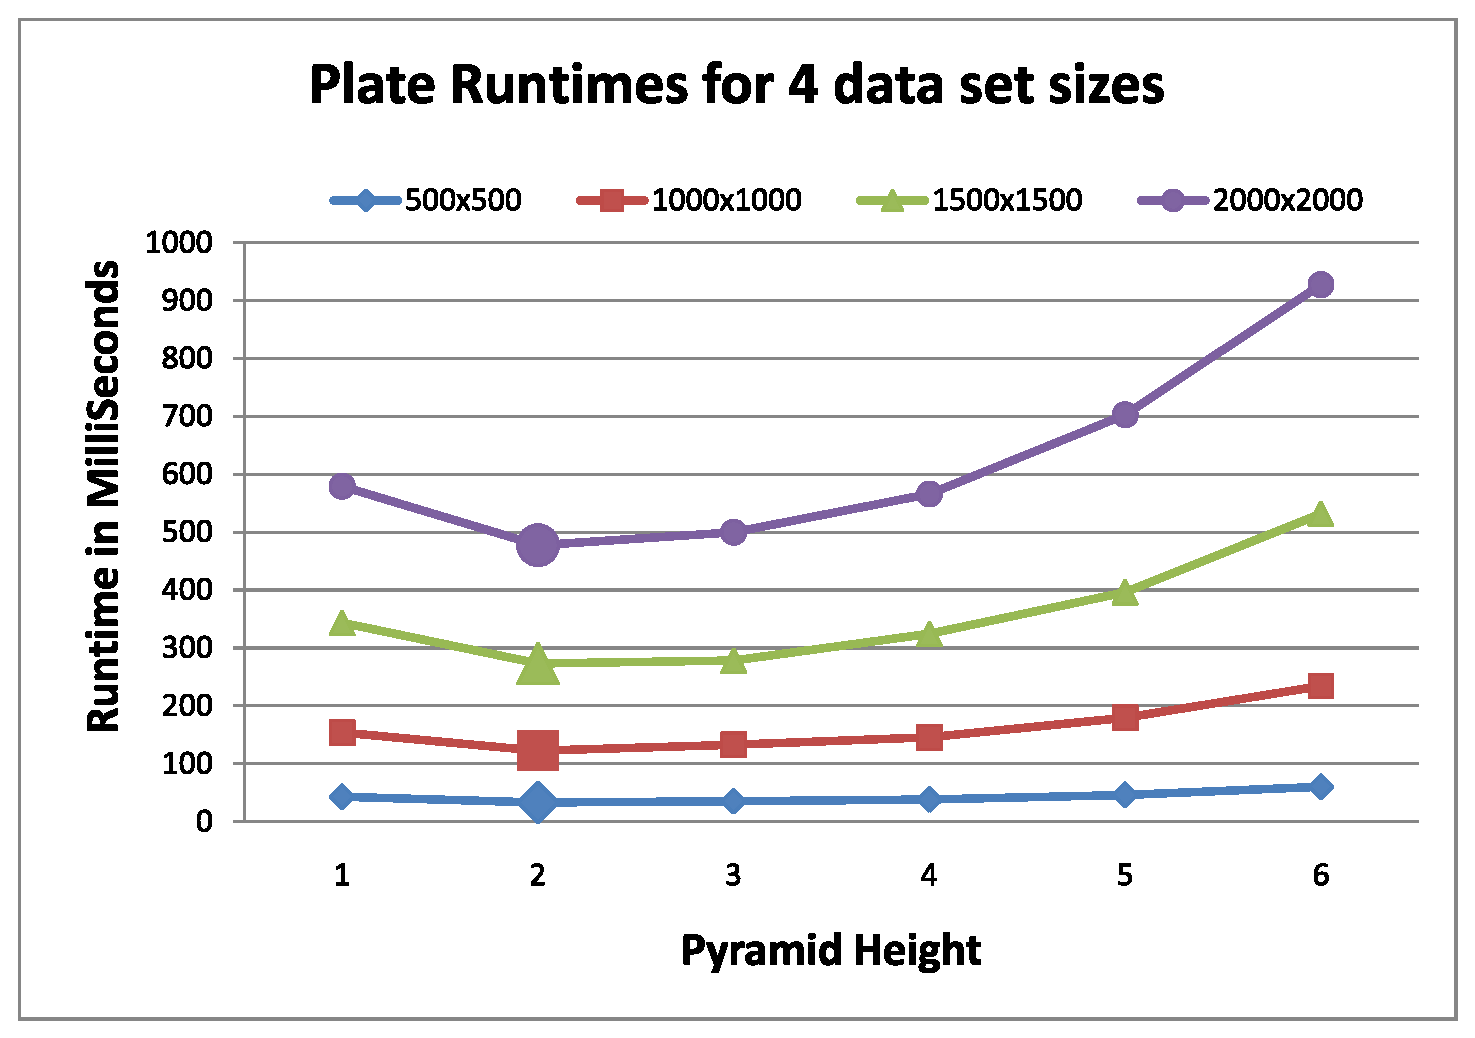
\includegraphics[clip,trim=1in 1in 1in 1in,width=3.3in]{PlateTimingData}
\caption{This chart shows the actual measured runtimes for the Plate 2D stencil application vs. PH.
The shape of the curve is very similar to HotSpot in spite of the difference is global read-only data access
and the use of an EdgeValue clause in the SL description.  Our optimizer picked the correct PH of 2 for all these data sets.}
\label{fig:plateTimes}
\end{figure}

\subsection{\em ``Cell''}
The fourth test case is a 3D stencil application called {\em ``Cell''}.  It models Conway's game of life in 3 dimensions.  
In each time step, each cell calculates whether it is alive or dead based on the number of neighboring cells that were alive in the previous
time step.  To perform this calculation, it looks at its 26 nearest neighbors.  For a 3D application, the current maximum tile size is 8x8x8, 
and the possible PHs are only 1 2 and 3.  The runtimes vs. PH are shown in Figure~\ref{fig:cellTimes}.  
It is very clear from the chart that a PH of 3 is a very bad choice.  The runtimes for PHs of 1 and 2 are closer, 
but 1 in better and is also predicted by our model.

\begin{figure}
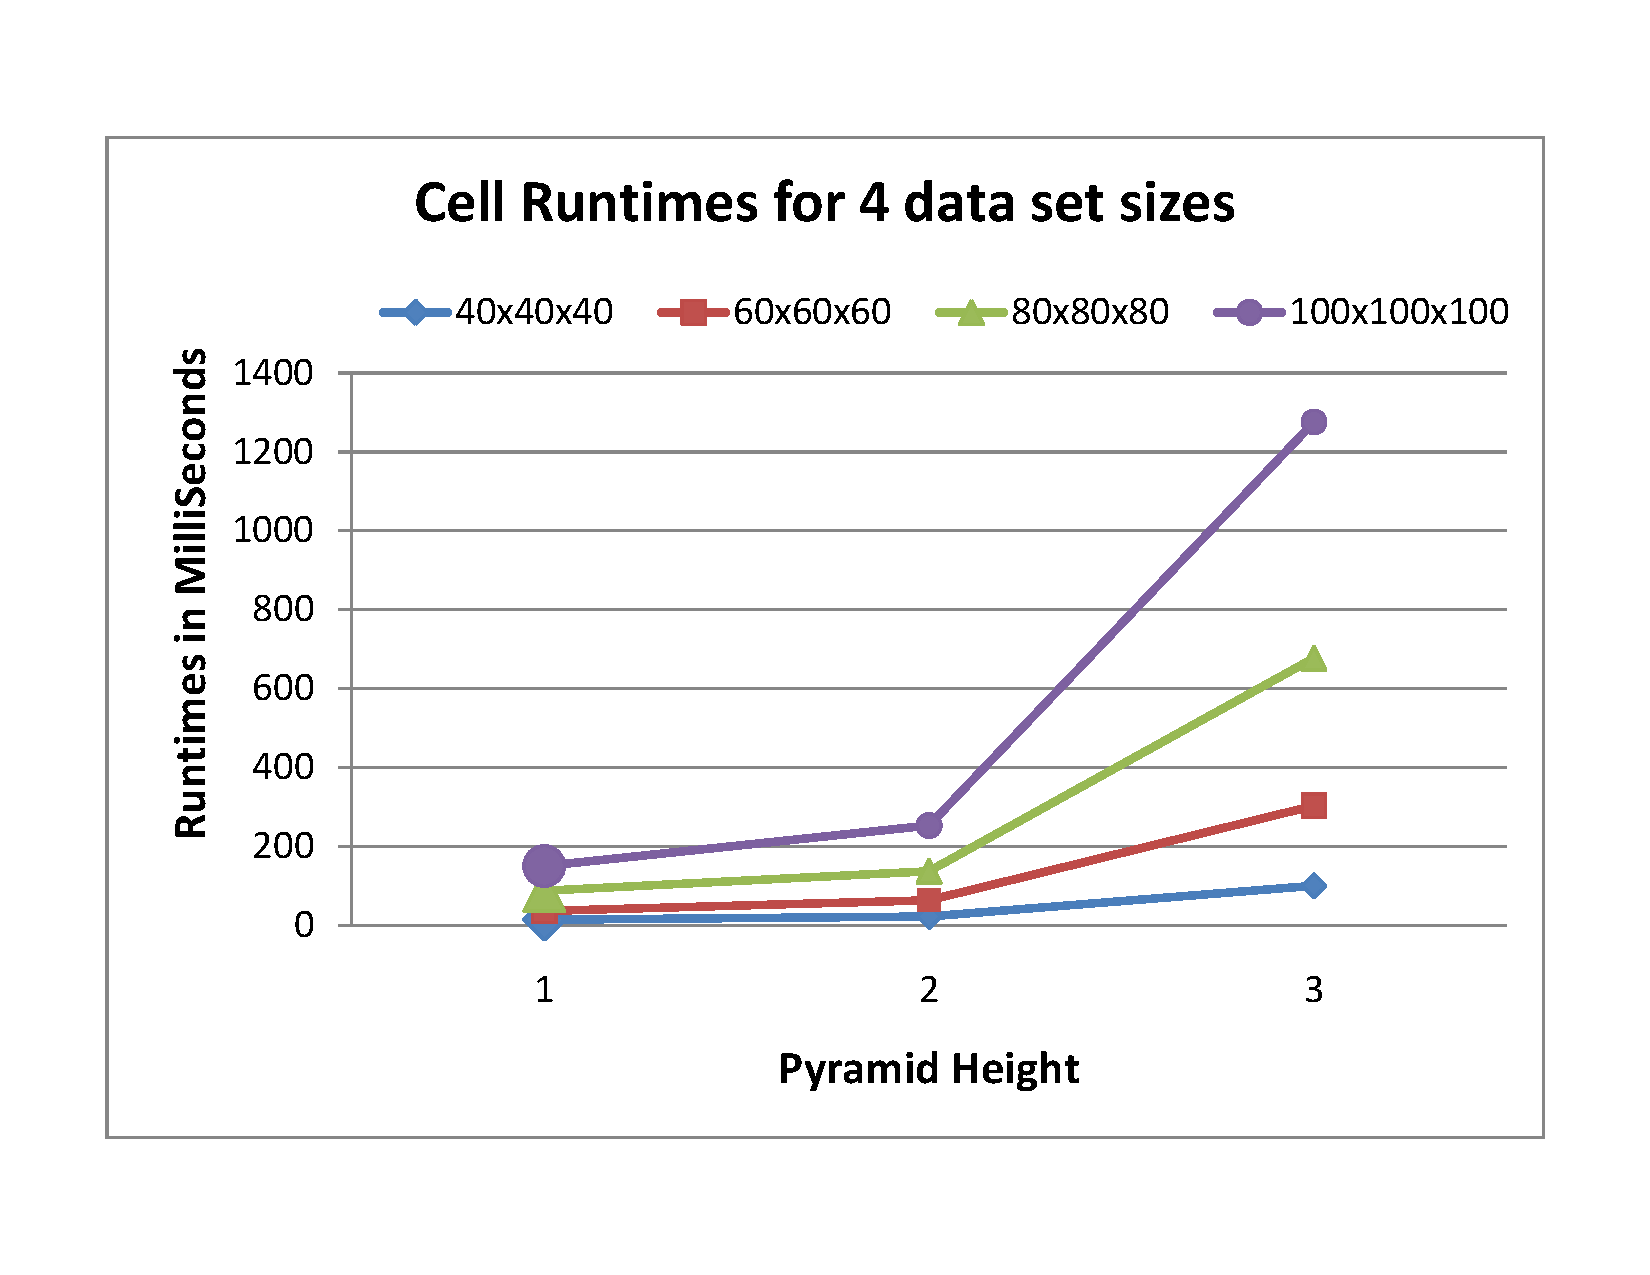
\includegraphics[clip,trim=1in 1in 1in 1in,width=3.3in]{CellTimingData}
\caption{This chart shows the actual measured runtimes for the Cell 3D stencil application vs. PH.
The curve shows that a PH of 3 is a very bad choice.  While the values for 1 and 2 are slightly 
compressed in the graph the optimal PH is in fact 1 for all data sets, as was accurately predicted by our optimizer.}
\label{fig:cellTimes}
\end{figure}

\subsection{Analysis}
As can be seen from the above, our model predicts the optimal PH for all shown data set sizes for HotSpot, Plate, and Cell.
These were the same PHs predicted by Meng's original model for these same applications and data set sizes.  However, he measured 
an optimal PH of 3 for HotSpot and Poisson.  His application implementations differ from ours in a three important ways.  

First, he used a tile size of 20x20 for these two applications in spite of the fact that our studies (as well as intuition) 
show larger tile sizes are always better.  It is unclear why he chose a tile size of 20x20.  
Second, as his applications were hand optimized,
he was able to load the read-only heat data used in HotSpot into shared memory to take advantage of temporal locality.  Our SL has no way to express
the access patterns for read-only data, and therefore our version of HotSpot will read the value from global memory in each time step.

Finally, his inner loop code calculates the cell values for all cells in the tile, even those that have become too far away from the center of the
tile to matter to the computation.  That is, tile cells that are completely surrounded by ghost cells.  Instead, our implementation recalculates the zone
of cells involved in useful computation on each time step.  This keeps threads from calculating values that will never be used.  This is particularly important
if read-only data is used as it is in HotSpot and Pathfinder.

\begin{figure}
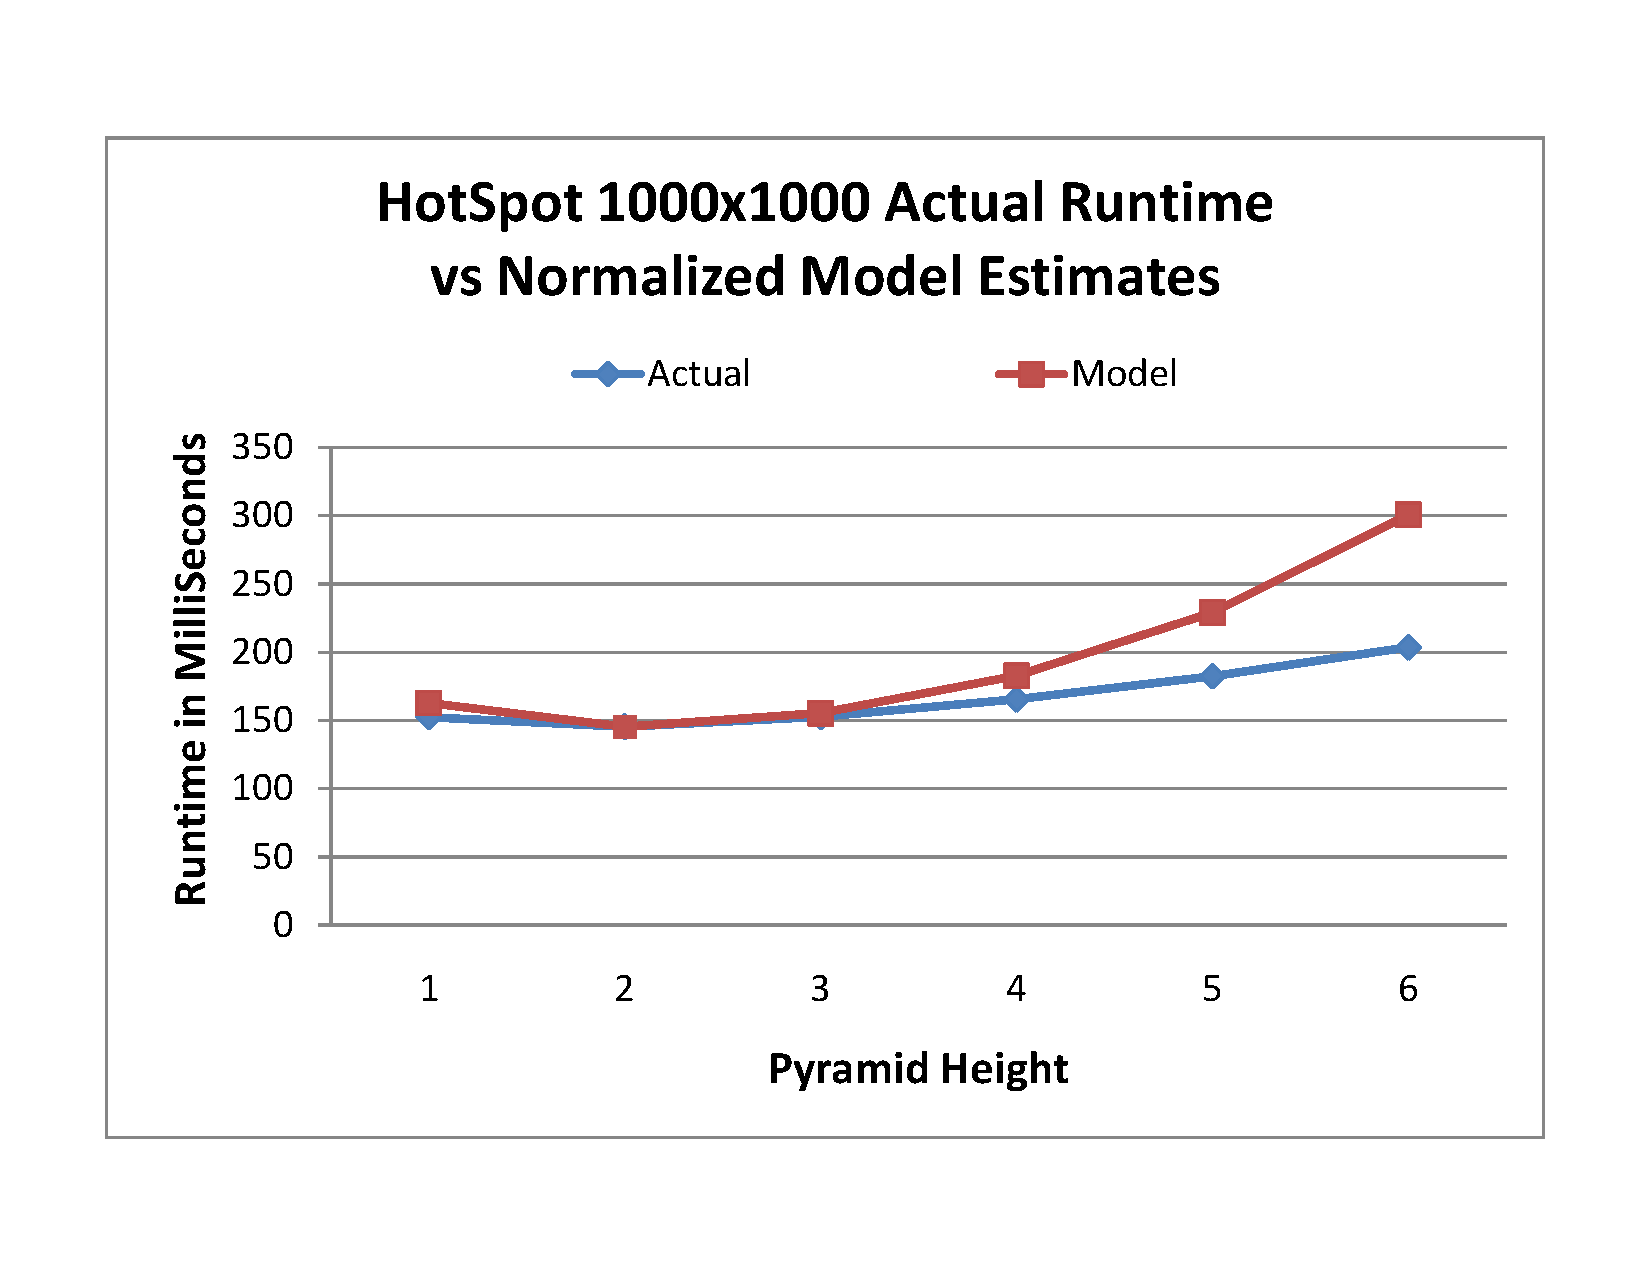
\includegraphics[clip,trim=1in 1in 1in 1in,width=3.3in]{HotSpotModelActual}
\caption{This chart shows the actual measured runtimes for HotSpot vs. the Model predicted 
The curve shows that a PH of 3 is a very bad choice.  While the values for 1 and 2 are slightly 
compressed in the graph the optimal PH is in fact 1 for all data sets, as was accurately predicted by our optimizer.}
\label{fig:modelvsactual}
\end{figure}

In the case of Pathfinder, for the 1,000,000 column data set size, Meng's original 
model properly calculated the optimal PH of 14, and his implementation
of Pathfinder also was optimal as a height of 14.  Instead, our implementation also performs best at height 14 in spite of 
the fact that we use a tile size of 512 vs. the 256 that Meng et al. used.  However, as state above, our model predicted a height of 19 which resulted
in a less than 1\% performance degradation.

The results presented her validate that the changes that we have made to the CUDA ISA predictive model have certainly not made it worse.
Given the elimination of the users' manual involvement in this optimization, we believe this to be an important contribution of this work.

We also analyzed the differences in the shape of the curves for actual runtime data vs. the model predictions.  
Figure~\ref{fig:modelvsactual} shows actual runtimes for HotSpot vs. the predicted runtimes from our model for 
PHs from 1 to 6.  The model times are normalized to equal the actual runtime at the optimal height of two.
This allows a more direct comparison of the shapes of the curves.  The actual Model predictions are in terms of GPU cycles,
not runtimes.  In addition, for the purposes of picking an optimal PH, the absolute scaling is not important,
but instead depends on the relative shapes of the curves.  As can be seen in the Figure, the model has a steeper bowl shape
than the actual runtimes.  The effect is more pronounced for higher PHs, and really grow large quickly for PHs 
between 6 and 10 which were excluded from the figure to better show the shapes of the curve in the most interesting part of the graph.


\section{Next Steps}

While substantial progress has been made during this project, 
there are a number of additional tasks that would further the research goals.  
These include the following:

\begin{enumerate*}
\item Use optimizer training period to do first few iterations of the application's work.
\item Improve support in SL for read-only data.  At least in the common cases such as HotSpot,
the read-only data should be moved into shared memory as the read-write data is.
\item Validate the optimizer for more test cases.
This would include additional applications that have not been used with the
model previously.  Also, testing should occur on more CUDA devices.  
We have made some preliminary tests of the model on other devices than the one reported here.  
While these results show early promise, they were not sufficiently complete to include in this
report.  We would also like to compare the optimization results against applications generated
through other means.  For example, we would like to compare against a naive CUDA implementations of
the sample stencil applications that use neither shared memory, nor ghost zones.  
Finally, we feel it would be interesting to test our optimized code 
against the results of applying CUDA-lite optimizations to the naive CUDA implementations.
Theoretically, the CUDA-lite optimizations should result in run-times similar to our
implementation used with a PH of 1.  This should be verified.
\item Validate the ability to target different parallel architectures by building a back-end
that generates OpenMP code.  In addition, since OpenMP in turn can generate code for many different parallel
architectures, this would offer the SL user a wide variety of target runtime environments.
\end{enumerate*}

\section{Conclusion}

The contributions of this project are as follows:
\begin{itemize*}
\item We have defined a new language, SL, for easily expressing
  stencil applications.  This is a formal high-level language 
  in which a programmer can describe an ISL
  computation.  The SL specification for a stencil application
  is focused on the simple computation needed to compute cell values.
  No optimization nor architectural specific information is included.
\item We have created a stencil language compiler.  
  The use of templates for the code generated by
  our compiler allows it to be extended to many
  parallel execution environments.  
  Based on a single source file, it could output efficient code for 
  CUDA or OpenMP or pthreads or other environments.
\item We have implemented an initial template and an optimizer
  for the CUDA programming environment.  The optimizer is 
  fully automatic and utilizes both static and dynamic information
  about the applications.  It accurately calculates the optimal tile size and 
  pyramid heights for several test applications.  
  It is an extension to the model defined by Meng and Skadron.
\item The optimizer's ability to also take advantage of 
  dynamically acquired information about the runtime environment
  means that the generated code can be used on a variety of CUDA
  devices, including the potential for use with future GPU cards.
\end{itemize*}


\balance
\bibliographystyle{plain}
\bibliography{report}
\end{document}
